\RequirePackage[l2tabu, orthodox]{nag}
\documentclass{article}

\usepackage[letterpaper, margin=1.3cm]{geometry}
\usepackage{siunitx}
\usepackage{multicol}
\usepackage{mathtools}
\usepackage{amssymb}
\usepackage{mathrsfs}
\usepackage{graphicx}
\usepackage{float}
\usepackage[outputdir=obj]{minted}
\usepackage{pdflscape}
\usepackage{caption}
\usepackage{subcaption}
\usepackage{epstopdf}
\usepackage{pgfplots}
\usepackage{pgfplotstable}
\usepackage{filecontents}

\epstopdfsetup{outdir=./obj/}
\usemintedstyle{emacs}
\setminted{linenos,breaklines}
\begin{filecontents*}{convolution.dat}
    0 0
    1 2
    2 5
    3 8
    4 10
    5 2
    6 -3
    7 -4
    8 0
\end{filecontents*}

\begin{document}

\begin{titlepage}
    \begin{center}
        \vspace*{1cm}

        \huge{\textbf{Lab 2}}

        \vspace{0.5cm}

        \LARGE{Convolution and Aliasing}
        \vspace{5cm}

        \Large{\textbf{Michael Kwok (1548454)}}

        \vfill
        ECE 340 Discrete Time Signals and Systems\\
        Department of Electrical and Computer Engineering\\
        University of Alberta\\
        12 October 2020
    \end{center}
\end{titlepage}
\begin{multicols}{2}
    \section{Convolution}
    \subsection{Pure Signal Convolution}
    \begin{figure}[H]
        \centering
        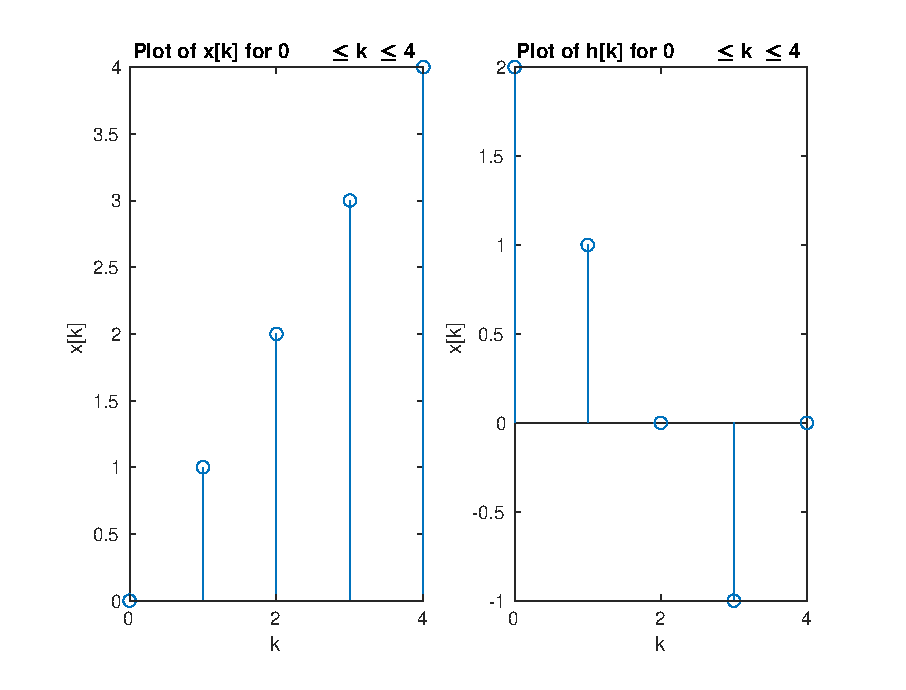
\includegraphics[width=\linewidth]{plot1}
        \caption{}
    \end{figure}
    \begin{figure}[H]
        \centering
        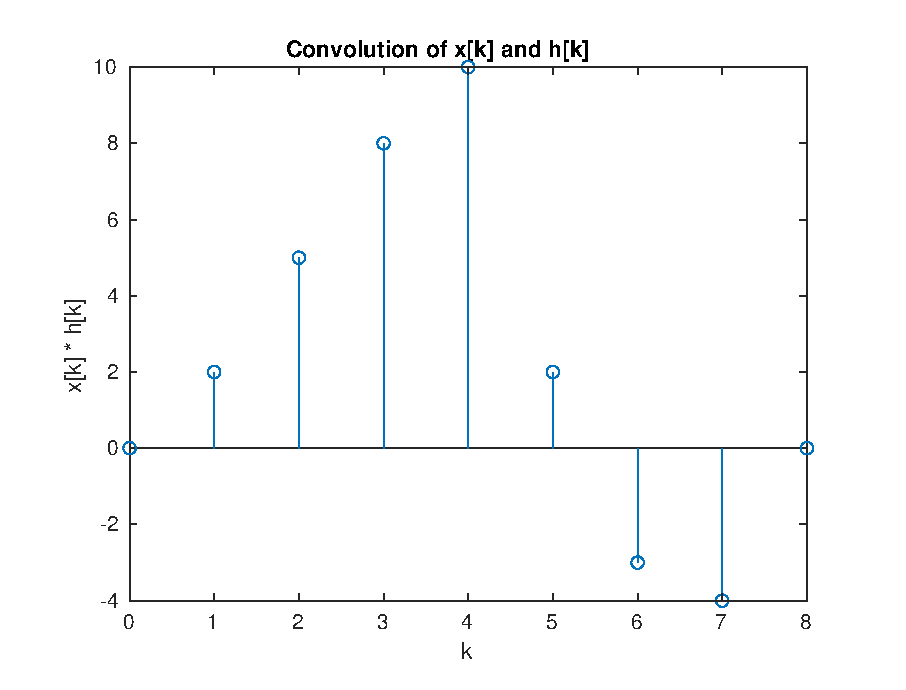
\includegraphics[width=\linewidth]{plot2}
        \caption{}
    \end{figure}
    \subsubsection{Convolution verification}
    \begin{align*}
        \sum_{n=-\infty}^\infty & h[n]x[k-n]                           \\
                                & = h[0]x[k] + h[1]x[k-1] + h[2]x[k-2] \\
                                & +h[3]x[k-3] + h[4]x[k-4]
    \end{align*}
    \begin{center}
        \begin{tabular}{| c | c c c c c c c c c | }
            \hline
            n            & 0 & 1 & 2 & 3 & 4  & 5  & 6  & 7  & 8 \\
            \hline
            \(2 x(n)\)   & 0 & 2 & 4 & 6 & 8  & 0  & 0  & 0  & 0 \\
            \(x(n-1)\)   & 0 & 0 & 1 & 2 & 3  & 4  & 0  & 0  & 0 \\
            \(- x(n-3)\) & 0 & 0 & 0 & 0 & -1 & -2 & -3 & -4 & 0 \\
            \hline
            \( \sum \)   & 0 & 2 & 5 & 8 & 10 & 2  & -3 & -4 & 0 \\
            \hline
        \end{tabular}
    \end{center}
    \begin{figure}[H]
        \centering
        \begin{tikzpicture}
            \begin{axis}[grid=major]
                \addplot+[ycomb] plot table[x index=0, y index=1]{convolution.dat};
            \end{axis}
        \end{tikzpicture}
        \caption{Result of manual convolution of \(x[k] \text{ and } h[k]\)}
    \end{figure}
    The two graphs match up, hence convolution verified.

    \subsection{Audio Convolution}
    \begin{figure}[H]
        \centering
        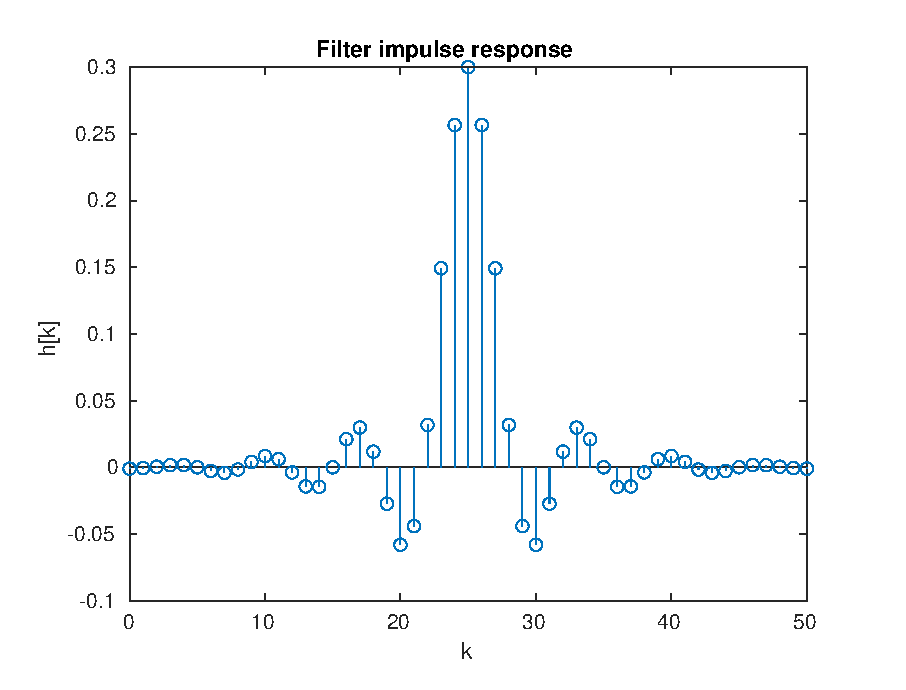
\includegraphics[width=\linewidth]{plot3}
        \caption{}
    \end{figure}
    Audio sounds less clear, more muddy. This is due to the application of the filter. The resulting audio is around double the size, which means the sample rate for the saved file is about double too.
    \subsection{Code}
    \begin{minted}{Matlab}
% Set output domain
k1 = [0:4];

% Use lambda functions to make definition shorter
x1 = @(n) (n) .* ((0 <= n) & (n <= 4));
h1 = @(n) (2 - n) .* ((0 <= n) & (n <= 3));

% Use built in convolution function
y = conv(x1(k1), h1(k1));
    \end{minted}

    \section{Signal Aliasing}
    \subsection{Pure Signal Aliasing}
    \begin{figure}[H]
        \centering
        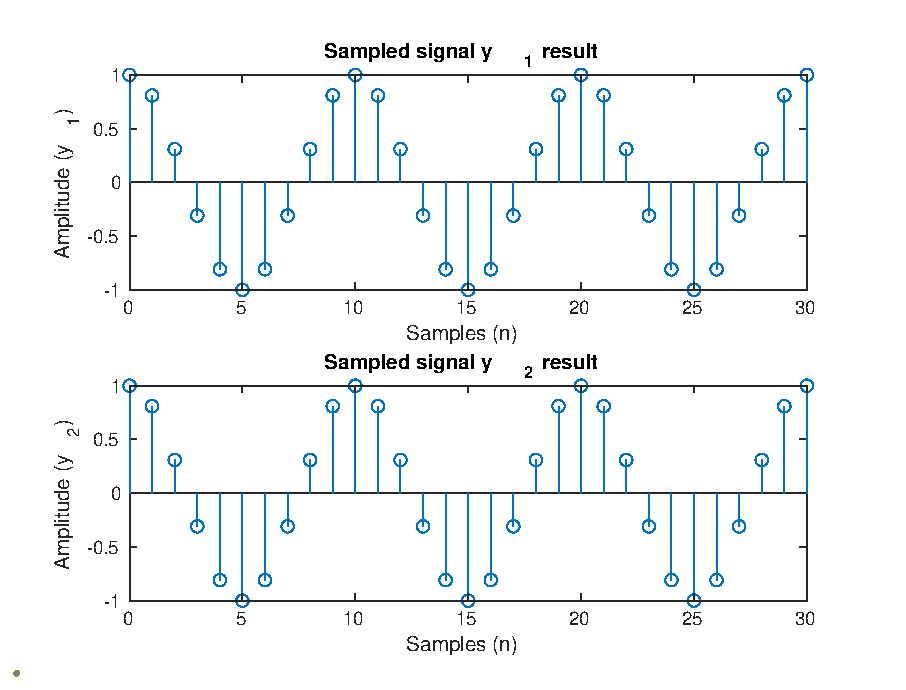
\includegraphics[width=\linewidth]{plot4}
        \caption{\(\cos(20\pi t)\) (top) vs \(\cos(180\pi t)\) (bottom) at \SI{100}{\hertz} }
    \end{figure}
    The plot of both signals look exactly the same. This is due to aliasing.
    \begin{align*}
        y_1[n] & = \cos\left(\frac{20\pi}{100}n\right) \\
               & = \cos\left(0.2\pi n\right)           \\
        y_2[n] & = \cos\left(1.8\pi n\right)           \\
               & = \cos\left(2\pi n- 0.2\pi n\right)   \\
               & = \cos\left(-0.2\pi n\right)
    \end{align*}
    Using the fact that \(\cos(-\theta) = \cos(\theta)\):
    \[y_2[n]  = \cos\left(-0.2\pi n\right) = \cos(0.2\pi n) = y_1[n]\]

    Which shows that \(y_2\), when sampled at the specified frequency of \SI{100}{\hertz} results in the same signal as \(y_1\), which is the definition of aliasing.

    Contrasted to the signals when they get sampled at \SI{1000}{\hertz}:
    \begin{figure}[H]
        \centering
        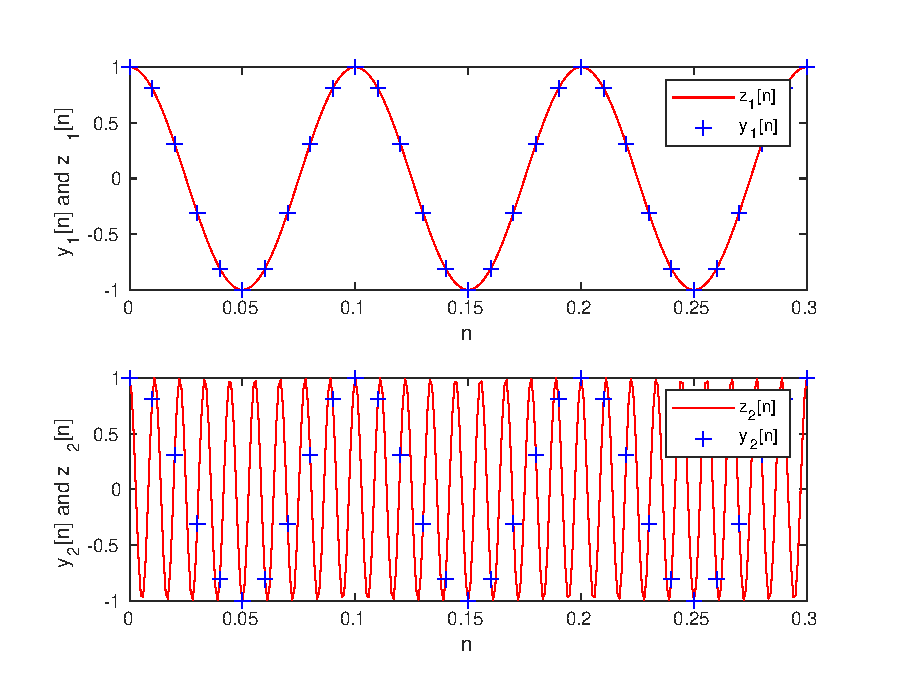
\includegraphics[width=\linewidth]{plot5}
        \caption{\(z_n\) are the respective \(y_n\) signals sampled faster}
    \end{figure}

    At \SI{100}{\hertz}, the higher frequency signal gets aliased as the lower frequency result, while at 1000 Hz, the higher frequency signal shows the more correct result.

    Other coeffecients of \(t\) in the continuous \( \cos \) can also be used to show aliasing. One of them is \( 380\pi \) as shown below:
    \begin{align*}
        y_1[n] & = \cos\left(0.2\pi n\right)             \\
        y_3[n] & = \cos\left(0.2\pi n + 2 N \pi n\right)
    \end{align*}
    Substitute \(N\) with any integer such as \(-2\) in this case:
    \begin{align*}
        y_3[n] & = \cos\left(0.2\pi n -4\pi n\right) \\
               & = \cos\left(3.8 \pi n \right)
    \end{align*}
    Convert back into a continuous unsampled function with \( n = F_s t\)
    \begin{align*}
        x_3(t) & = \cos\left(3.8 \pi \cdot 100 \cdot t \right) \\
               & =\cos\left(380 \pi t \right)
    \end{align*}
    \begin{figure}[H]
        \centering
        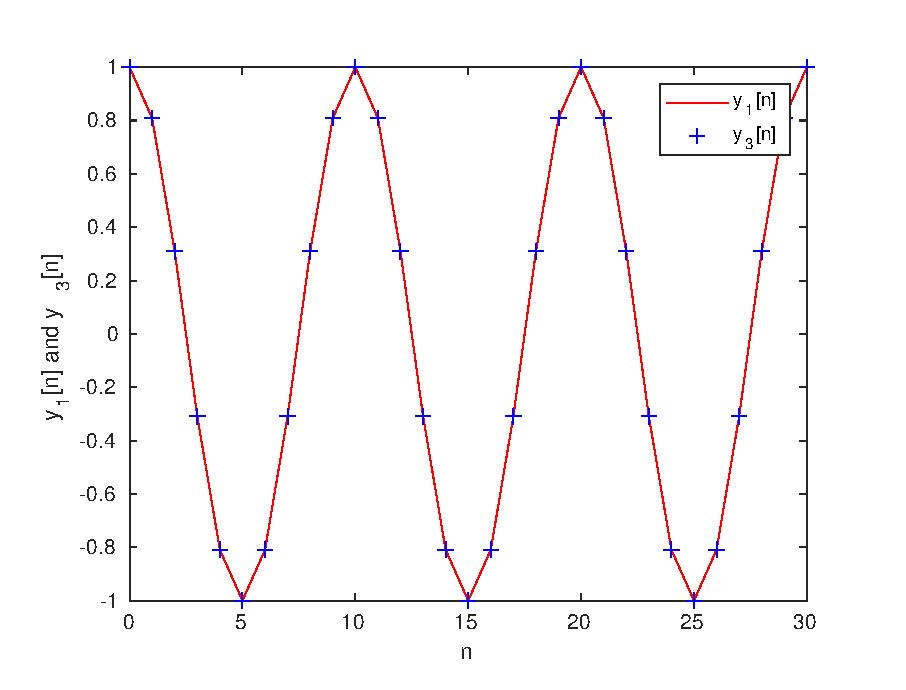
\includegraphics[width=\linewidth]{plot6}
        \caption{Another possible signal that can be aliased to \(y_1\)}
    \end{figure}
    \subsubsection{Code}
    \begin{minted}{Matlab}
% Part a
n1 = [0:30]';
x1 = @(t) (cos(20 .* pi .* t));
x2 = @(t) (cos(180 .* pi .* t));

T1 = 1 / 100;

y1 = x1(T1 .* n1);
y2 = x2(T1 .* n1);

% Part b
n2 = [0:300];
T2 = 1 / 1000;
z1 = x1(T2 .* n2);
z2 = x2(T2 .* n2);

% Part c
x3 = @(t) (cos(380 .* pi .* t));
y3 = x3(T1 .* n1);
        \end{minted}
\end{multicols}
\subsection{Image Aliasing}
\begin{figure}[H]
    \centering
    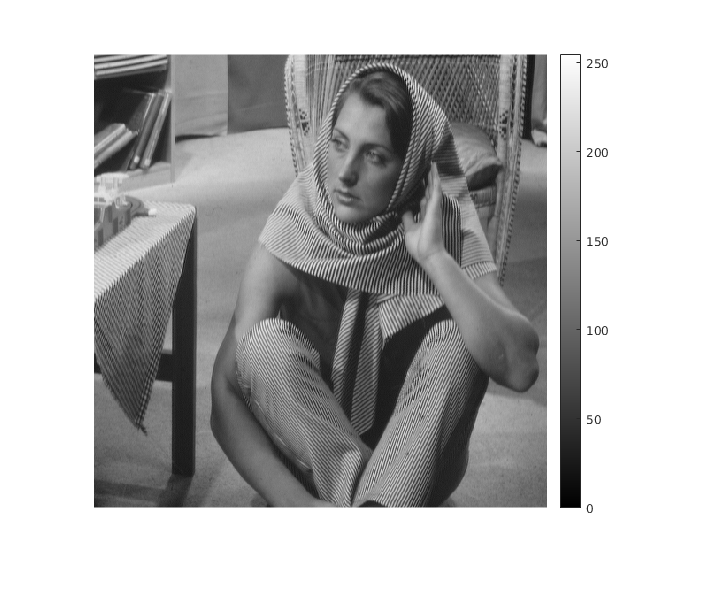
\includegraphics[width=0.8\linewidth]{barb_bar.png}
    \caption{barbaraLarge.jpg with a brightness bar on the side}
\end{figure}
\begin{figure}
    \centering
    \begin{subfigure}[b]{0.4\linewidth}
        \centering
        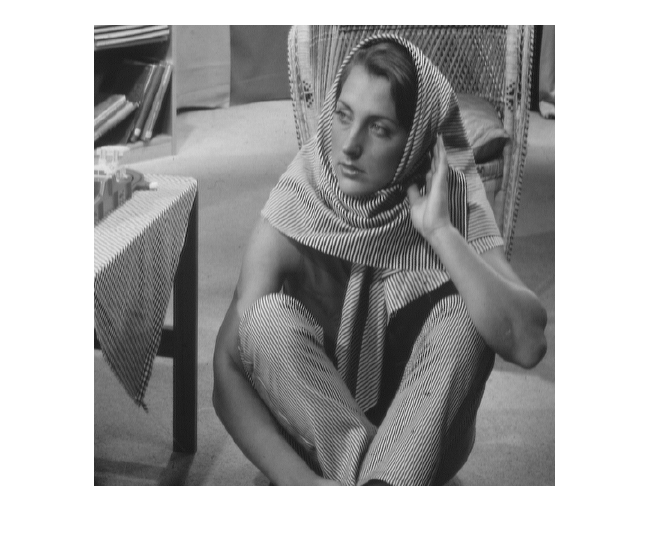
\includegraphics[width=\linewidth]{barb09aa.png}
        \caption{barbaraLarge.jpg downscaled by 0.9 with antialiasing}
    \end{subfigure}
    \begin{subfigure}[b]{0.4\linewidth}
        \centering
        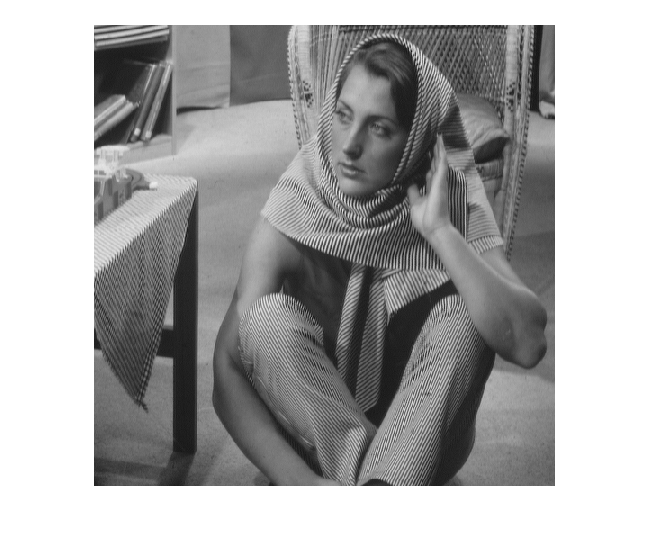
\includegraphics[width=\linewidth]{barb09noaa.png}
        \caption{barbaraLarge.jpg downscaled by 0.9 without antialiasing}
    \end{subfigure}
    \begin{subfigure}[b]{0.4\linewidth}
        \centering
        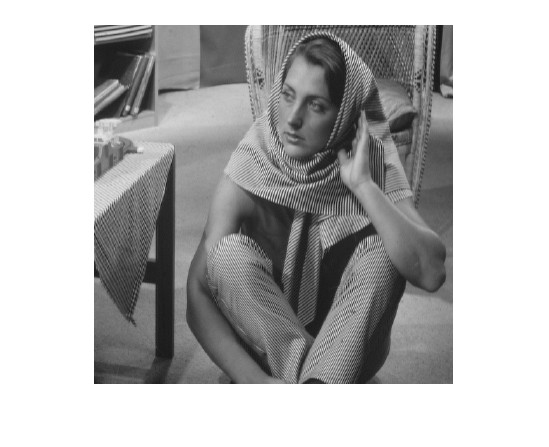
\includegraphics[width=\linewidth]{barb07aa.png}
        \caption{barbaraLarge.jpg downscaled by 0.7 with antialiasing}
    \end{subfigure}
    \begin{subfigure}[b]{0.4\linewidth}
        \centering
        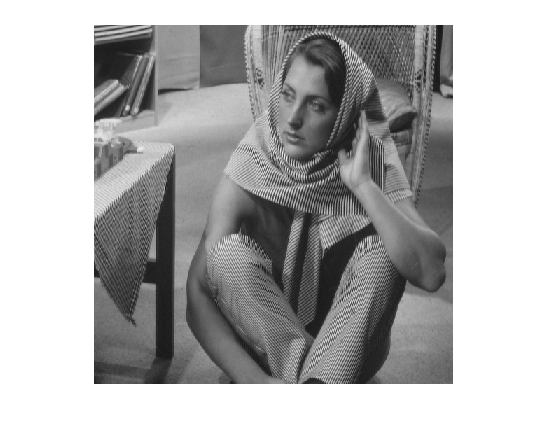
\includegraphics[width=\linewidth]{barb07noaa.png}
        \caption{barbaraLarge.jpg downscaled by 0.7 without antialiasing}
    \end{subfigure}
    \begin{subfigure}[b]{0.4\linewidth}
        \centering
        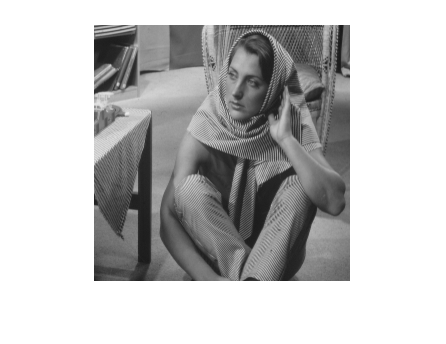
\includegraphics[width=\linewidth]{barb05aa.png}
        \caption{barbaraLarge.jpg downscaled by 0.5 with antialiasing}
    \end{subfigure}
    \begin{subfigure}[b]{0.4\linewidth}
        \centering
        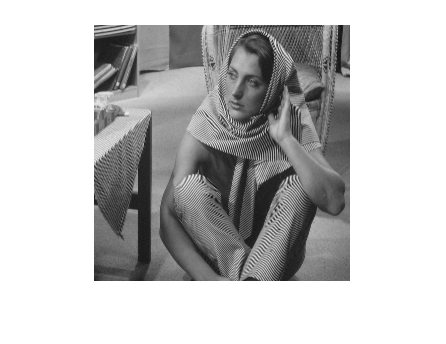
\includegraphics[width=\linewidth]{barb05noaa.png}
        \caption{barbaraLarge.jpg downscaled by 0.5 without antialiasing}
    \end{subfigure}
    \caption{All scaled figures}
\end{figure}

The floor behind the person stays unchanged despite all the downscaling, due to it being mostly ``random noise'' and not ordered lines. The tablecloth, pants and headscarf all have lines that due to the compression algorithm was aliased into different lines. The direction of the lines seem to be change in every image. Sharp edges such as the table leg's line down also lose defintion as the image size is reduced. The frequency of which the image is sampled (``resolution'') is reduced as the image scale gets smaller, which explains all the above. The antialiased versions of every picture is smoother than the non-antialiasing versions, which could be due to application of a low pass filter, reducing the high frequency pixel data.


Downscaled images on next page.
\subsubsection{Code}
\begin{minted}{Matlab}
%% Question 4 Image Aliasing
% Part a
img = imread('barbaraLarge.jpg');

% Part c
img09aa = imresize(img, 0.9, 'nearest', 'antialiasing', 1);
img09noaa = imresize(img, 0.9, 'nearest', 'antialiasing', 0);

img07aa = imresize(img, 0.7, 'nearest', 'antialiasing', 1);
img07noaa = imresize(img, 0.7, 'nearest', 'antialiasing', 0);

img05aa = imresize(img, 0.5, 'nearest', 'antialiasing', 1);
img05noaa = imresize(img, 0.5, 'nearest', 'antialiasing', 0);
\end{minted}
\pagebreak
\appendix
\section{Complete Code (lab2.m)}
\inputminted{Matlab}{lab2.m}
\end{document}
